%************************************************
\section{Session tracking}\label{p02:session_tracking}
%************************************************

In order to understand the learning process, we need to keep track of the working sessions. The term refers to either reading or exercising sessions. A reading session is considered as an uninterrupted reading activity of a particular article, while an exercise session can encompass multiple articles. Given the fact that students can switch between windows or even walk away from the screen, a method to compute the effective working time is devised. 

\subsection{Algorithm}
Working sessions are computed under the assumption that all user actions fall into one out of three types: opening, interaction or closing events.

By following the Markov model on figure \ref{fig:markov_diagram}, we observe that depending on the type of event, a working session can be either created, updated (kept alive) or closed. With this simple approach, the algorithm can be fine tuned by adding or removing events (\eg, including the scrolling as a interaction event).

\begin{figure}[bth]
	{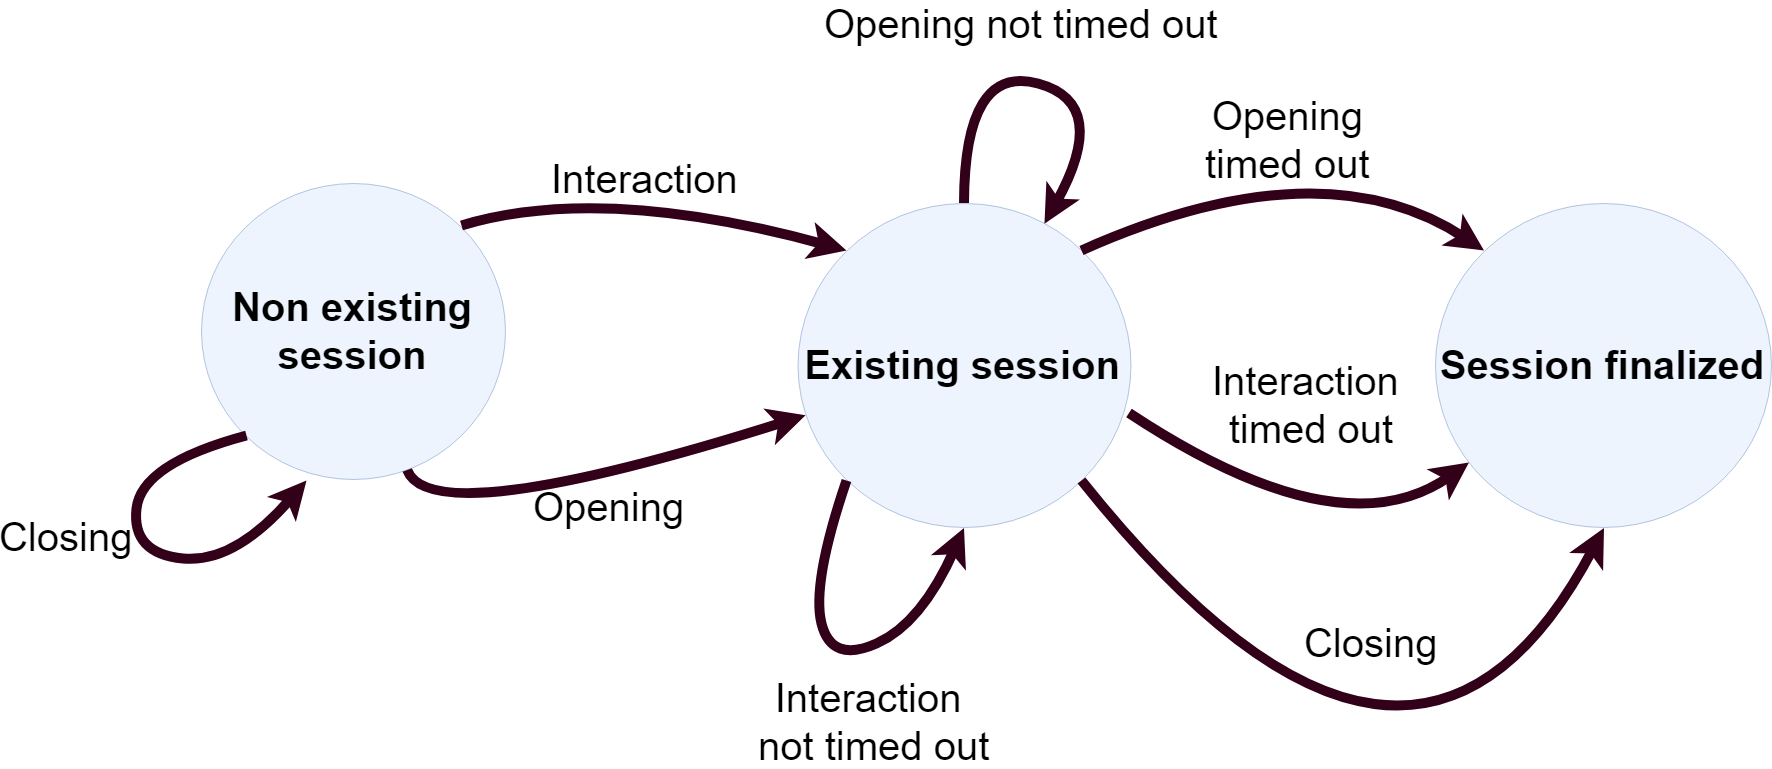
\includegraphics[width=1\linewidth]{gfx/Finite_state_machine_diagramv2}} \quad
	\caption[Finite state diagram - Working session transitions due to user actions]{Finite state diagram - Working session transitions due to user actions}\label{fig:markov_diagram}
\end{figure}

Additionally, there is a \textbf{session\_timeout} parameter which is used to handle scenarios where a session was not properly closed (\eg, when the browser was closed or the computer was turned off). The parameter is used in 2 different situations:

\begin{itemize}
	\item When the user is inactive for a long period, the session is closed and a bonus of \textbf{session\_timeout} minutes are added to the last action date and time. Under the assumption that the user did not stop working immediately after the last action.
	
	\item When the user is taking unusually too long between actions the activity is considered as suspicious and the session is closed. A new session is created with the next user action.
\end{itemize}

For the specific case of Zeeguu platform, the implementation of the algorithm is divided in two layers: front and back ends. The front end is implemented in Javascript and it tracks the user actions with the system. The back end is implemented in python and is where the logic for the working sessions is implemented.

Figure \ref{fig:session_tracking_architecture} shows the architecture of the implementation. As we can observe, the implementation is divided in two layers, which means that they can work independently. Therefore the user actions can be tracked in real time, while the algorithm that computes the sessions can be run on a separate batch, thus leveraging the workload. The modules can also work in real time if the tracking module triggers the execution of the session stitching module.

Relevant user actions are detected by the front end layer of the system, and stored in the database. The back end periodically retrieves the list of user events and stitches them or creates a new session depending on the type of event and the time between the actions. Therefore inserting the session information back in the database, making it available to be displayed.
The front end layer can also trigger the execution of the session stitching module after each user activity, enabling real time session analysis.

%TODO include layers diagram
\begin{figure}[bth]
	\centering
	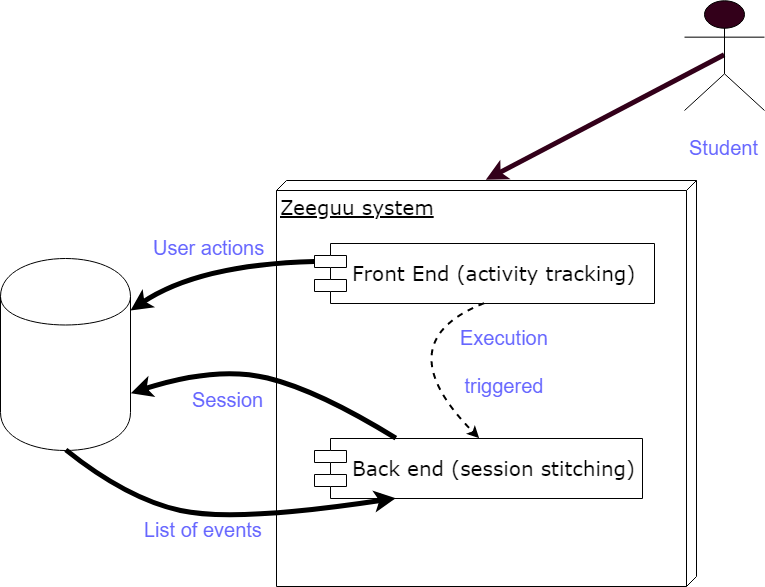
\includegraphics[width=0.7\linewidth]{gfx/session_tracking_architecture}
	\caption{Session tracking architecture}\label{fig:session_tracking_architecture}
\end{figure}

\subsection{Reading session}
For the reading session, Javascript listeners are used to track the following user events:
\begin{itemize}
	\item Open list of articles
	\item Open an article
	\item Translate a word
	\item Undo a word translation
	\item Lose and gain focus on the page
	\item Scrolling
	\item Close an article
\end{itemize}

When the information is detected, it is immediately stored in the database. Once the article is closed or a new article is opened, the backend triggers the events' \textit{stitching}, and the session is computed.

While defining what a session is in the system, and given the fact that the application is on the web, the following difficulties are encountered:
\begin{itemize}
	\item Events like closing the browser or turning off the computer cannot be detected
	\item If the user walks away from the screen, we cannot detect exactly when it was and if he read a couple of minutes before leaving
	\item The user can open multiple instances of Zeeguu, and each instance can have a different article open
	\item If the user opened multipe articles, the user can change from article to article in a short time period
	\item The user can be using more than one device at the same time
	\item The user can read an article in multiple sessions
\end{itemize}

Therefore the following assumptions for the implementation of the reading session are considered:
\begin{itemize}
\item Reading session are considered per article. Therefore, when the user closes and opens a new article we consider it as a new session. In this way we solve the issue where the same user could have opened different articles in different tabs and switches between them.

\item For scenarios when the user leaves the session open for a time period longer than the session\_timeout, we give it a time benefit of “session\_timeout” minutes, because we cannot know exactly how long after the last action, the user kept reading. 

\item A user is supposed to read one article at the time. Therefore, when the user opens a new article without closing the previous one(s) we close the other reading session(s)

\item A user can read the same article multiple times, and each time is considered a new session (unless the time between both of them is less than the session timeout, in which case the two sessions are merged).
\end{itemize}

As mentioned before, a timeout parameter is used for finalizing a session after \textbf{N} number of minutes. If the timeout value is too small an advanced student that does not translate any word but reads a long text might be incorrectly measured, while if the value is too big, we would incorrectly consider longer reading sessions. Therefore, defining the value of the timeout is crucial. 


\subsection{Exercise session}
For the exercise sessions, the front end layer starts a timer when the exercise is opened. When it is answered (either correct or incorrect) or a hint is requested, the event is stored in the database with the elapsed time.

The back end layer is immediately executed after the front end code, appending the recently answered exercise to the exercise session or creating a new one when the elapsed time is larger than the timeout value.

Therefore, opening an exercise does not count for the active session, only answering.

For exercise sessions we can be more precise on the tracking because an exercise usually comes surrounded by a single sentence, therefore the timeout can be set to a smaller value. 

The final difference with the reading session is that no "benefit time" is granted to the user, the only actions that keep the session alive are answering the exercise.


%TODO explain events tracked and events that were added

%TODO explain script for historical data


%TODO Later, the implementation of the algorithm in the system, for this, it was needed to implement additional user actions detection (lost focus, and scrolling)